\documentclass[10pt, compress]{beamer}

\usetheme{m}

\usepackage{booktabs}
\usepackage[scale=2]{ccicons}
\usepackage{minted}

\usemintedstyle{pastie}

\title{Random number generation}
\subtitle{Quantitative Risk Management project work}
\date{}
\author{Silvia Baldisserotto, Maysa Jahanbani, \\ Claudia Pesci, Phan Ho Tan Phat, \\ Andrea Venuta}
\institute{Università degli Studi di Firenze - Finance and Risk Management}

\renewcommand{\theFancyVerbLine}{\sffamily \textcolor[rgb]{0.5,0.5,0.5}{\small \oldstylenums{\arabic{FancyVerbLine}}}}

\begin{document}

\maketitle

\begin{frame}[fragile]
  \frametitle{Random numbers}
  \begin{itemize}
  	\item Computer-generated numbers are \textit{pseudo-random}: deterministic and predictable
  	\item \textit{Quasi-random} numbers prevent potential lack of equidistributedness
  	\item \textbf{Definition.} \textit{(sample)} a sequence of number is called a \textit{sample from the distribution $F$}
  	  if the numbers are independent realizations of a random variable with distribution function $F$
	\item Uniform deviates: samples from $\sim \mathcal{U}  \left[ 0, 1 \right] $
	\item Normal deviates: samples from $\sim \mathcal{N}  \left( 0, 1 \right) $
	\item Drawing uniform deviates is the basis of random number generation
  \end{itemize}
\end{frame}

\begin{frame}[fragile]
  \frametitle{Linear congruential generators}
  	\begin{itemize}
  	  \item $N_0$ is chosen arbitrarily (called the \textit{seed})
  	  \item $N_i = (aN_{i-1} + b)\ \text{mod}\ M$ for $i > 0$
  	  \item \[U_i = \frac{N_i}{M},\quad U_i \in \left[0,1\right)\]
  	  \item Suitability of the numbers $U_i$ depends on how $a, b, M$ are chosen
  	\end{itemize}
\end{frame}

\begin{frame}[fragile]
  \frametitle{Linear congruential generators: properties}
  \begin{itemize}
    \item Numbers $N_i$ are periodic, with period $\leq M$: there are at most $M$ different numbers in the class modulo $M$
    \item Example: if $N=0$, $b$ can't be $0$, otherwise $N_i = 0$ will repeat itself
    \item Example: if $a=0$, generator settles down on $N_n = N_0 + nb$
    \item Numbers are distributed ``evenly'' if we have exactly $M$ different numbers in a generator with modulo $M$, or
    \item Each grid point on a \textit{mesh} on $\left[0,1\right]$ with \textit{mesh} size $\frac{1}{M}$ is occupied once
  \end{itemize}
\end{frame}

\begin{frame}[fragile]
  \frametitle{Quality of generators}
  Requirements:
  \begin{enumerate}
  	\item Large period: small set of numbers makes the outcome easier to predict (choose M as large as possible)
  	\item Statistical tests to verify that the distribution is the intended one
  	  \begin{itemize}
  	  	\item Comparison of sample mean and variance $\mu,\ \sigma^2$ with desired values
  	  	\item Correlation between sample values
  	  	\item Quality of approximation of the distribution
  	  \end{itemize}
     \item Distribution in higher dimensional spaces: lattice structure
  \end{enumerate}
\end{frame}

\begin{frame}[fragile]
  \frametitle{Random vectors and lattice structure}
  \begin{itemize}
  	\item Sequences of random numbers can be arranged in $m$-dimensional vectors
  	\item The vectors lie on a number of parallel $(m-1)$-dimensional hyperplanes
  	\item The ideal condition is that the number of parallel hyperplanes is maximized:
  	  number of hyperplanes is a measure of equidistributedness
  	\item Family of parallel lines in the $(U_{i-1},U_i)$-plane \[
  		z_0 U_{i-1} +z_1 U_i = c + \frac{z_1 b}{M} \quad \text{where} \quad c := N_{i-1}\frac{z_0 + az_1}{M} - z_1 k
  	  \] for each tuple $(z_0,z_1)$ and for all $c$s.
  \end{itemize}
\end{frame}

\begin{frame}[fragile]
  \frametitle{Random vectors and lattice structure}
  immagini qui
\end{frame}

\begin{frame}[fragile]
  \frametitle{Inversion and transformation methods}
  \begin{itemize}
  	\item Inversion and transformation methods generate numbers distributed according to
  	  an arbitrary distribution from uniformly distributed samples
  \end{itemize}
\end{frame}

\begin{frame}[fragile]
  \frametitle{Box-Muller method}
  \begin{itemize}
  	\item Generate $x_1, x_2 \sim \mathcal{U}(0,1)$ random numbers
  	\item Derive
  	  \[ h_1(x_1, x_2) := y_1 = \sqrt{-2 \log x_1} \cos{2\pi x_2} \]
  	  \[ h_2(x_1, x_2) := y_2 = \sqrt{-2 \log x_1} \sin{2\pi x_2} \] 
	\item $y_1$ and $y_2$ will be i.i.d. $\sim \mathcal{N}(0,1)$
  \end{itemize}
\end{frame}

\begin{frame}[fragile]
  \frametitle{Box-Muller method}
  \begin{columns}[t]
    \begin{column}{4cm}
	  %\includegraphics[width=.8\textwidth]{Picture1.png}
    \end{column}
    \begin{column}{4cm}
      \[ y_1 = D \cos \omega \quad y_2 = D \sin \omega \quad \]
      \[ \text{where}\ D = \sqrt{-2 \log x_1} \quad \omega = 2\pi x_2 \]
    \end{column}
  \end{columns}

  \bigskip
  
  \bigskip
  
  \[
    h^{-1}(x_1,x_2) = \begin{cases}
      x_1 = \exp{\left\{ -\frac{y_1^2 + y_2^2}{2} \right\}}       
      \\
      x_2 = \frac{1}{2\pi} \arctan \frac{y_2}{y_1}
    \end{cases}
  \]
  \[
  	|\text{Jacobian}| = \det \left(
  	  \begin{matrix}
  	    \frac{\partial x_1}{\partial y_1} & \frac{\partial x_1}{\partial y_2} \\
  	    \frac{\partial x_2}{\partial y_1} & \frac{\partial x_2}{\partial y_2} 
  	  \end{matrix}
  	\right) = 
  	\left[ 
  	  \frac{1}{\sqrt{2\pi}} \exp{\left(-\frac{y_1^2}{2}\right)}
  	\right]
  	\cdot
  	\left[
  	  \frac{1}{\sqrt{2\pi}} \exp{\left(-\frac{y_2^2}{2}\right)} 
  	\right]
  \]
  is the density of the bivariate standard normal distribution because it's the product of two univariate standard normal densities.
\end{frame}

\begin{frame}[fragile]
  \frametitle{Polar method}
  \begin{enumerate}
    \item Let $U_1, U_2 \sim \mathcal{U}(0,1)$
    \item Define $V_i = 2U_i - 1$: $V_i \sim \mathcal{U}(-1,1)$
    \item Define $S = V_1^2 + V_2^2$
    \item If and only if $S \leq 1$, then define
      \[ Y = \sqrt{\frac{-2\ln{S}}{S}} \]
    \item \[
        \left( \begin{matrix} X_1 \\ X_2 \end{matrix} \right) = \left( \begin{matrix} V_1 Y \\ V_2 Y \end{matrix} \right)
        \quad \text{ and } \quad X_1,X_2\ \text{i.i.d.}\ \sim \mathcal{N}(0,1)
      \]
  \end{enumerate}  
\end{frame}

\begin{frame}[fragile]
  \frametitle{Polar method}
  \includegraphics[width=\textwidth]{Picture2.png}
\end{frame}

\begin{frame}[fragile]
  \frametitle{Correlated bivariate random variables}
  \[
    \mathbf{Z} = \left(\begin{matrix} z_1 \\ z_2 \end{matrix} \right), \quad z_1, z_2 \sim \mathcal{N}(0,1)
    \quad
    \mathbf{\mu} = \left(\begin{matrix} \mu_1 \\ \mu_2 \end{matrix} \right)
    \quad
    \Sigma = \left(\begin{matrix} \sigma_1^2 & \rho\sigma_1\sigma_2 \\ \rho\sigma_1\sigma_2 & \sigma_2^2 \end{matrix} \right)
  \]
  \begin{enumerate}
    \item Calculate the Cholesky decomposition $AA^T = \Sigma$
      \[
        \left(\begin{matrix} a & 0 \\ b & c \end{matrix} \right)
        \left(\begin{matrix} a & b \\ 0 & c \end{matrix} \right) =
        \left(\begin{matrix} a^2 & ab \\ ab & b^2 + c^2 \end{matrix} \right)
        = \left(\begin{matrix} \sigma_1^2 & \rho\sigma_1\sigma_2 \\ \rho\sigma_1\sigma_2 & \sigma_2^2 \end{matrix} \right)
      \] \[
        \rightarrow A = \left(\begin{matrix} \sigma_1 & 0 \\ \rho\sigma_2 & \sigma_2(1-\rho^2)^{\frac{1}{2}} \end{matrix} \right)
      \]
    \item Calculate $\mathbf{Z} \sim\mathcal{N}(0,\mathbb{I}_2)$
    \item $\mu + A\mathbf{Z} \sim \mathcal{N}(\mu,\Sigma)$ has the desired distribution.
      \[
        \left( \begin{matrix}X \\ Y \end{matrix} \right) = 
        \mu + %\left( \begin{matrix}\mu_1 \\ \mu_2 \end{matrix} \right) + 
          \left(\begin{matrix} \sigma_1 & 0 \\ \rho\sigma_2 & \sigma_2(1-\rho^2)^{\frac{1}{2}} \end{matrix} \right)
          \left(\begin{matrix} z_1 \\ z_2 \end{matrix} \right) =
        \mu + % \left( \begin{matrix}\mu_1 \\ \mu_2 \end{matrix} \right) + 
          \left(\begin{matrix} \sigma_1 z_1 \\ \rho\sigma_2z_1+\sigma_2(1-\rho^2)^\frac{1}{2}z_2 \end{matrix} \right)
      \]
  \end{enumerate}
\end{frame}

\begin{frame}[fragile]
	\frametitle{Implementations - Linear Congruential Generator}
	\begin{columns}[t]
		\begin{column}{5cm}
	
			\begin{minted}[fontsize=\small,linenos]{matlab}
function [ rn ] = LCG( x ) 

  if(nargin == 0)
    x = 1;
  end
  
  rn = zeros(x,1);
  
  for i = 1:x
    rn(i) = LCGstep();
  end

end
			\end{minted}
		\end{column}
		\begin{column}{5cm}
			\begin{minted}[fontsize=\small,linenos,firstnumber=14]{matlab}
function [ rnStep ] = LCGstep()

  persistent seed;
  M = 244944;
  a = 1597;
  b = 51749;
  
  if(isempty(seed))
    seed = 0;
  end
  
  seed = mod(seed * a + b, M);
  
  rnStep = seed / M;

end
			\end{minted}
		\end{column}
	\end{columns}
\end{frame}

\begin{frame}[fragile]
	\frametitle{Implementations - Box-Muller method}
	\begin{minted}[fontsize=\small,linenos]{matlab}
function [ Z ] = BoxMuller( x )

  if(nargin == 0)
    x = 1;
  end

  U = rand(x, 2);
  
  theta = 2 .* pi .* U(:, 2);
  rho   = sqrt( -2 .* log( U(:, 1) ) );
  
  Z = [ rho .* cos(theta), rho .* sin(theta) ];

end
	\end{minted}
\end{frame}

\begin{frame}[fragile]
	\frametitle{Implementations - Marsaglia polar algorithm}
	\begin{minted}[fontsize=\small,linenos]{matlab}
function [ Z ] = Marsaglia( x )

  if(nargin == 0)
    x = 1;
  end

  Z = zeros(x,2);
  
  for i = 1 : x
    W = 1;  V = [ 1, 1 ];
    while not (W < 1)
      V = 2 * rand(1, 2) - 1;
      W = V(1) .^ 2 + V(2) .^ 2;
    end
    
    Z(i, :) = V .* sqrt(-2 * log(W) / W);
  end
end
	\end{minted}
\end{frame}

\begin{frame}[fragile]
	\frametitle{Plots - Univariate methods}
	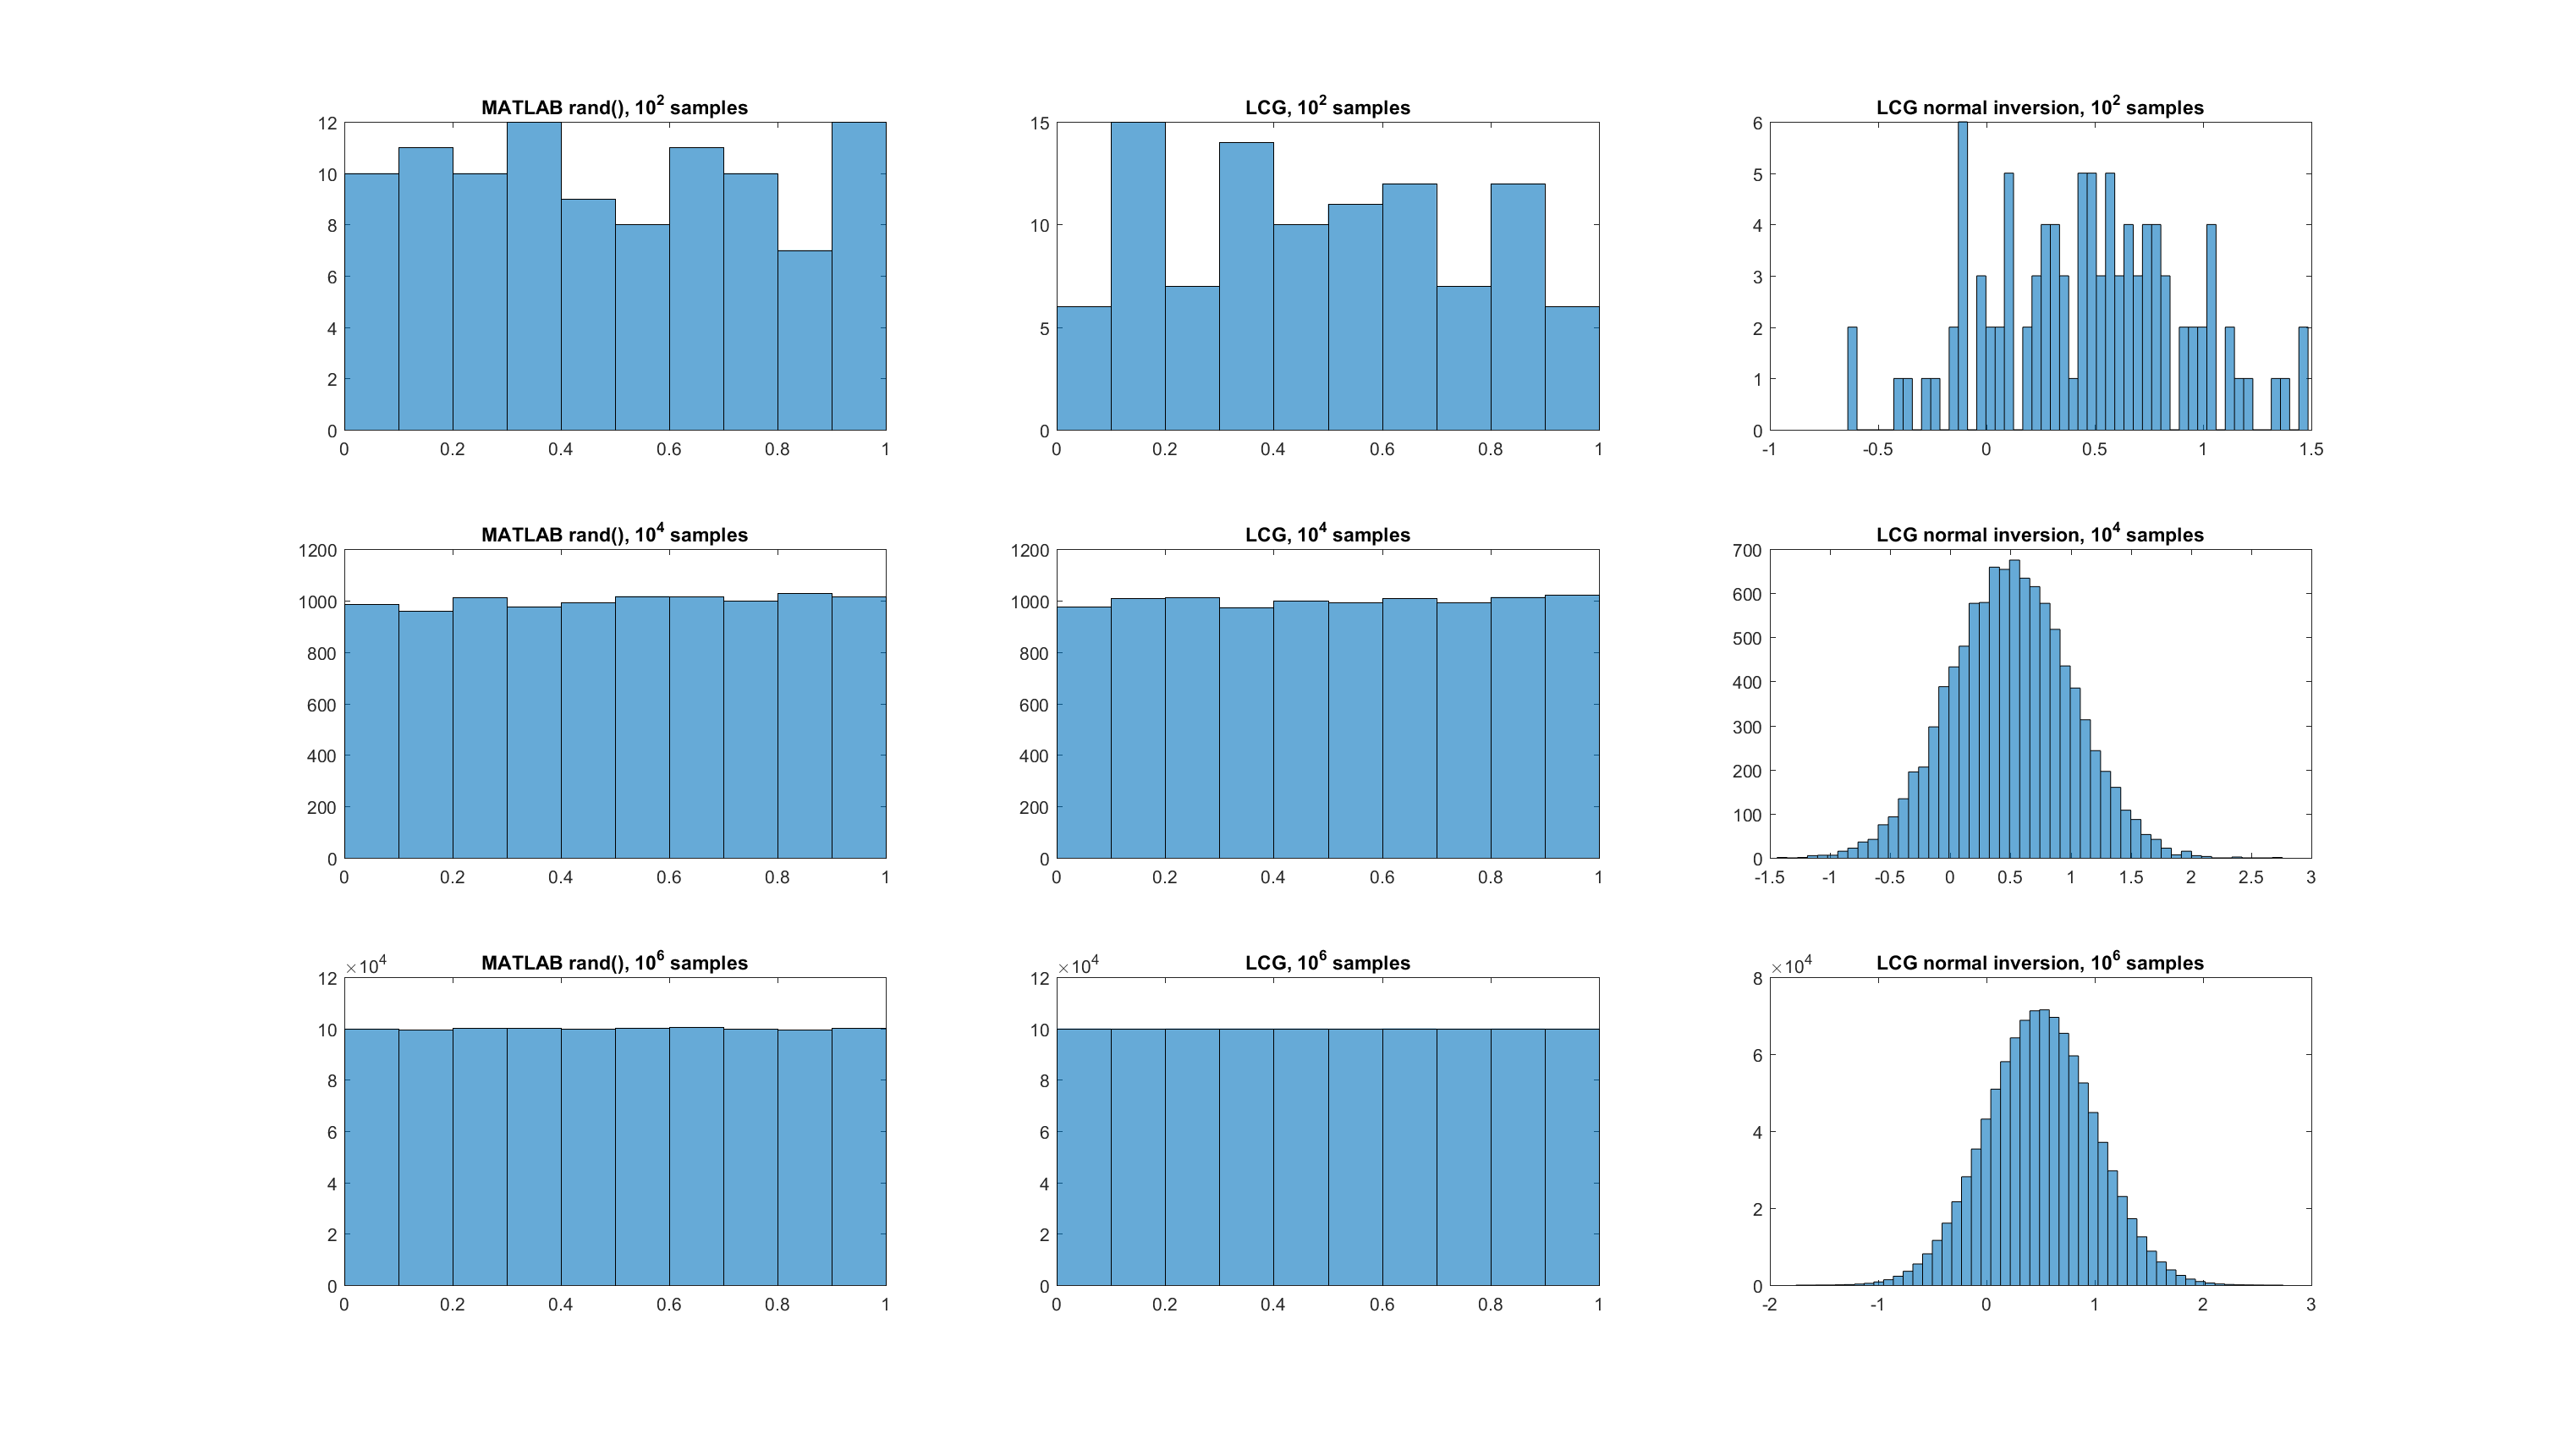
\includegraphics[width=\textwidth, trim=70mm 80mm 70mm 20mm]{../univariate.eps}
\end{frame}

\begin{frame}[fragile]
	\frametitle{Plots - Bivariate methods}
	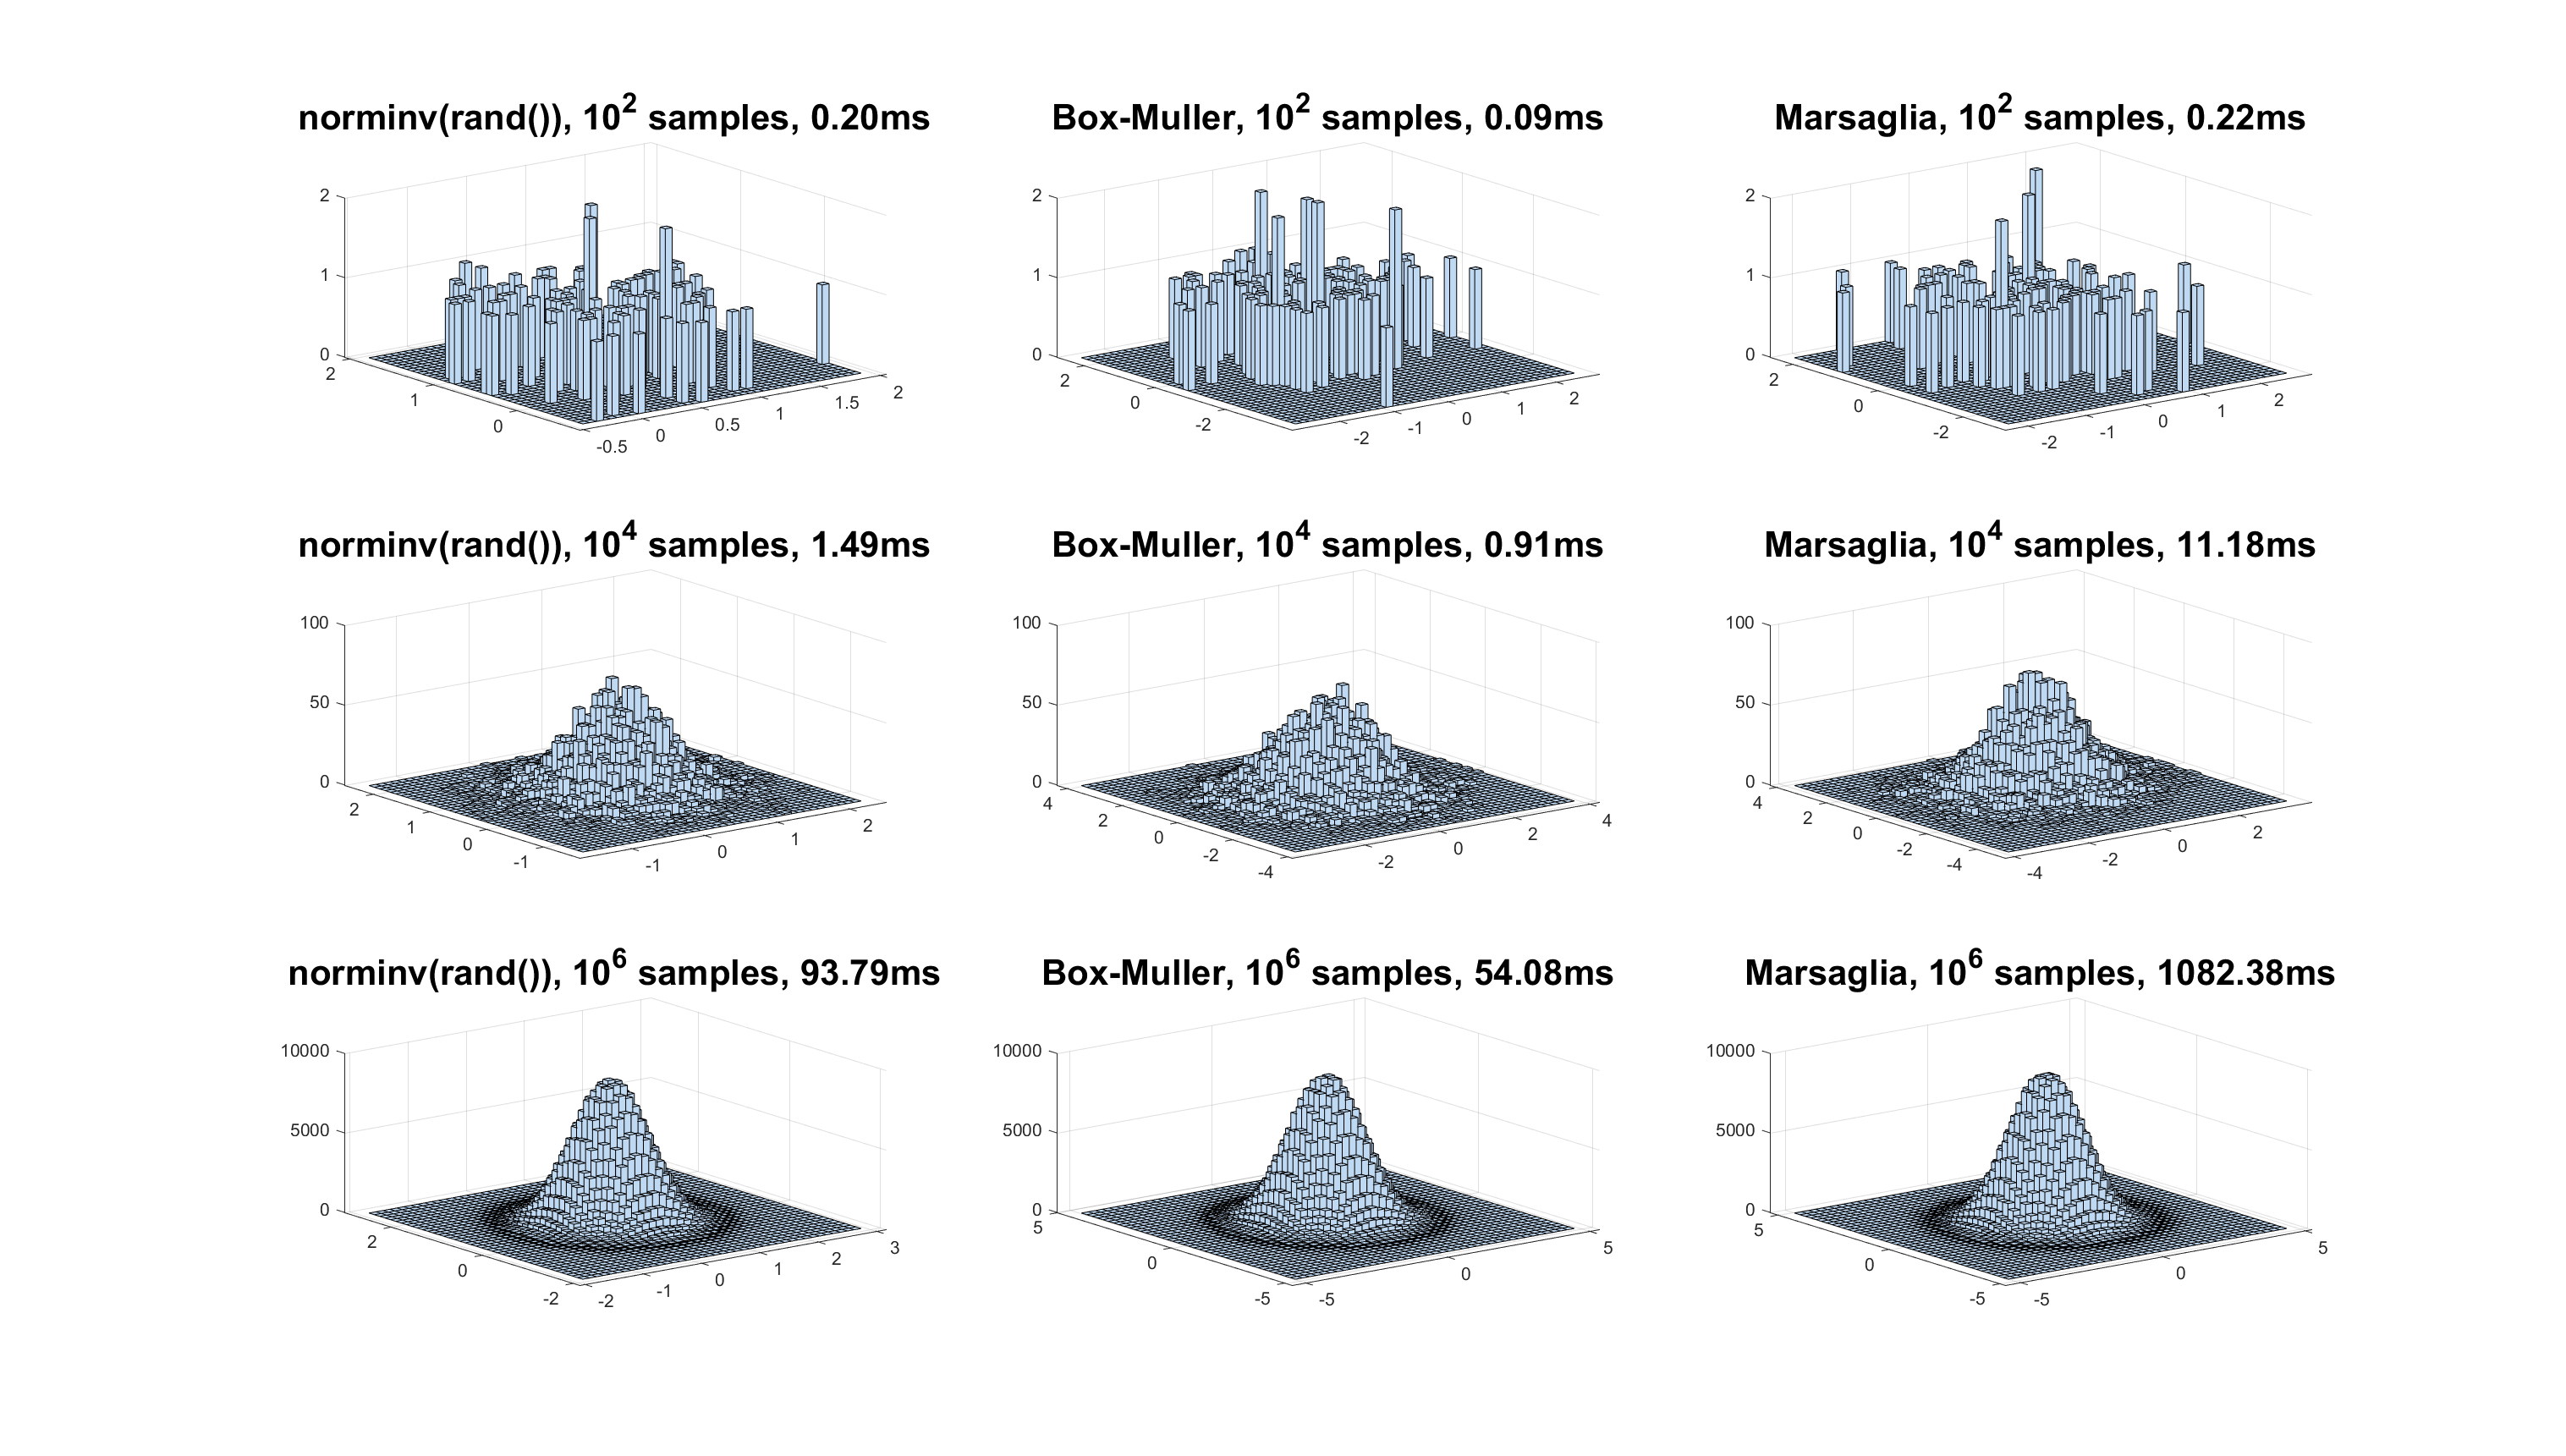
\includegraphics[width=\textwidth, trim=70mm 80mm 70mm 20mm]{../bivariate.eps}
\end{frame}

\end{document}
